\begin{wrapfigure}{l}{0.506\textwidth}
\vspace{-0.56cm}
\setlength{\abovecaptionskip}{0.3cm}
\setlength{\belowcaptionskip}{-0.3cm}
	\centering
    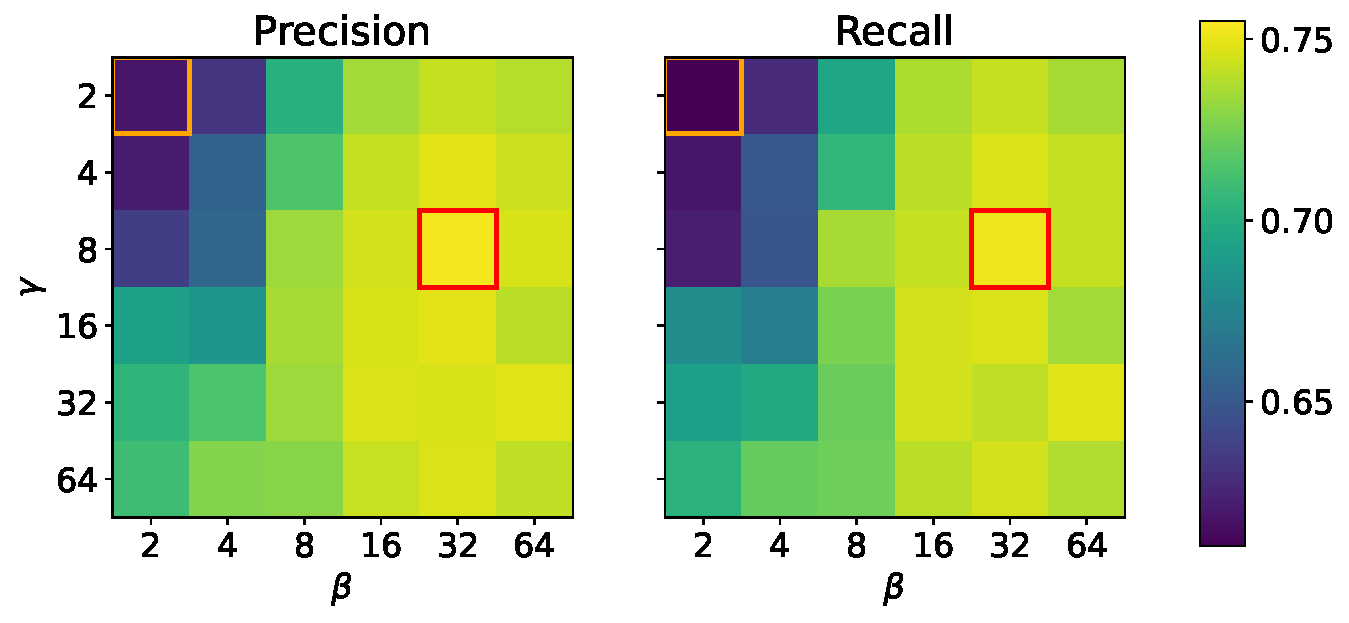
\includegraphics[width=\linewidth, trim={0cm 0cm 0cm 0cm},clip]{Figures/beta.pdf}
    \caption{\textbf{Weighted precision and recall for the binary classification task under varying Lagrange multipliers.} The graph shows the impact of varying the Lagrange multipliers ($\beta$ and $\gamma$). For each plot, the Red (Orange) color denotes the highest (lowest) value, respectively.}
    \label{fig:beta_dim}
\end{wrapfigure}